% Options for packages loaded elsewhere
\PassOptionsToPackage{unicode}{hyperref}
\PassOptionsToPackage{hyphens}{url}
\PassOptionsToPackage{dvipsnames,svgnames,x11names}{xcolor}
\documentclass[
  10pt,
]{extarticle}
\usepackage{xcolor}
\usepackage[top=1.25in, bottom=1.25in, left=1.25in, right=1.25in]{geometry}
\usepackage{amsmath,amssymb}
\setcounter{secnumdepth}{5}
\usepackage{iftex}
\ifPDFTeX
  \usepackage[T1]{fontenc}
  \usepackage[utf8]{inputenc}
  \usepackage{textcomp} % provide euro and other symbols
\else % if luatex or xetex
  \usepackage{unicode-math} % this also loads fontspec
  \defaultfontfeatures{Scale=MatchLowercase}
  \defaultfontfeatures[\rmfamily]{Ligatures=TeX,Scale=1}
\fi
\usepackage{lmodern}
\ifPDFTeX\else
  % xetex/luatex font selection
\fi
% Use upquote if available, for straight quotes in verbatim environments
\IfFileExists{upquote.sty}{\usepackage{upquote}}{}
\IfFileExists{microtype.sty}{% use microtype if available
  \usepackage[]{microtype}
  \UseMicrotypeSet[protrusion]{basicmath} % disable protrusion for tt fonts
}{}
\makeatletter
\@ifundefined{KOMAClassName}{% if non-KOMA class
  \IfFileExists{parskip.sty}{%
    \usepackage{parskip}
  }{% else
    \setlength{\parindent}{0pt}
    \setlength{\parskip}{6pt plus 2pt minus 1pt}}
}{% if KOMA class
  \KOMAoptions{parskip=half}}
\makeatother
\usepackage{color}
\usepackage{fancyvrb}
\newcommand{\VerbBar}{|}
\newcommand{\VERB}{\Verb[commandchars=\\\{\}]}
\DefineVerbatimEnvironment{Highlighting}{Verbatim}{commandchars=\\\{\}}
% Add ',fontsize=\small' for more characters per line
\usepackage{framed}
\definecolor{shadecolor}{RGB}{248,248,248}
\newenvironment{Shaded}{\begin{snugshade}}{\end{snugshade}}
\newcommand{\AlertTok}[1]{\textcolor[rgb]{0.94,0.16,0.16}{#1}}
\newcommand{\AnnotationTok}[1]{\textcolor[rgb]{0.56,0.35,0.01}{\textbf{\textit{#1}}}}
\newcommand{\AttributeTok}[1]{\textcolor[rgb]{0.13,0.29,0.53}{#1}}
\newcommand{\BaseNTok}[1]{\textcolor[rgb]{0.00,0.00,0.81}{#1}}
\newcommand{\BuiltInTok}[1]{#1}
\newcommand{\CharTok}[1]{\textcolor[rgb]{0.31,0.60,0.02}{#1}}
\newcommand{\CommentTok}[1]{\textcolor[rgb]{0.56,0.35,0.01}{\textit{#1}}}
\newcommand{\CommentVarTok}[1]{\textcolor[rgb]{0.56,0.35,0.01}{\textbf{\textit{#1}}}}
\newcommand{\ConstantTok}[1]{\textcolor[rgb]{0.56,0.35,0.01}{#1}}
\newcommand{\ControlFlowTok}[1]{\textcolor[rgb]{0.13,0.29,0.53}{\textbf{#1}}}
\newcommand{\DataTypeTok}[1]{\textcolor[rgb]{0.13,0.29,0.53}{#1}}
\newcommand{\DecValTok}[1]{\textcolor[rgb]{0.00,0.00,0.81}{#1}}
\newcommand{\DocumentationTok}[1]{\textcolor[rgb]{0.56,0.35,0.01}{\textbf{\textit{#1}}}}
\newcommand{\ErrorTok}[1]{\textcolor[rgb]{0.64,0.00,0.00}{\textbf{#1}}}
\newcommand{\ExtensionTok}[1]{#1}
\newcommand{\FloatTok}[1]{\textcolor[rgb]{0.00,0.00,0.81}{#1}}
\newcommand{\FunctionTok}[1]{\textcolor[rgb]{0.13,0.29,0.53}{\textbf{#1}}}
\newcommand{\ImportTok}[1]{#1}
\newcommand{\InformationTok}[1]{\textcolor[rgb]{0.56,0.35,0.01}{\textbf{\textit{#1}}}}
\newcommand{\KeywordTok}[1]{\textcolor[rgb]{0.13,0.29,0.53}{\textbf{#1}}}
\newcommand{\NormalTok}[1]{#1}
\newcommand{\OperatorTok}[1]{\textcolor[rgb]{0.81,0.36,0.00}{\textbf{#1}}}
\newcommand{\OtherTok}[1]{\textcolor[rgb]{0.56,0.35,0.01}{#1}}
\newcommand{\PreprocessorTok}[1]{\textcolor[rgb]{0.56,0.35,0.01}{\textit{#1}}}
\newcommand{\RegionMarkerTok}[1]{#1}
\newcommand{\SpecialCharTok}[1]{\textcolor[rgb]{0.81,0.36,0.00}{\textbf{#1}}}
\newcommand{\SpecialStringTok}[1]{\textcolor[rgb]{0.31,0.60,0.02}{#1}}
\newcommand{\StringTok}[1]{\textcolor[rgb]{0.31,0.60,0.02}{#1}}
\newcommand{\VariableTok}[1]{\textcolor[rgb]{0.00,0.00,0.00}{#1}}
\newcommand{\VerbatimStringTok}[1]{\textcolor[rgb]{0.31,0.60,0.02}{#1}}
\newcommand{\WarningTok}[1]{\textcolor[rgb]{0.56,0.35,0.01}{\textbf{\textit{#1}}}}
\usepackage{longtable,booktabs,array}
\usepackage{calc} % for calculating minipage widths
% Correct order of tables after \paragraph or \subparagraph
\usepackage{etoolbox}
\makeatletter
\patchcmd\longtable{\par}{\if@noskipsec\mbox{}\fi\par}{}{}
\makeatother
% Allow footnotes in longtable head/foot
\IfFileExists{footnotehyper.sty}{\usepackage{footnotehyper}}{\usepackage{footnote}}
\makesavenoteenv{longtable}
\usepackage{graphicx}
\makeatletter
\newsavebox\pandoc@box
\newcommand*\pandocbounded[1]{% scales image to fit in text height/width
  \sbox\pandoc@box{#1}%
  \Gscale@div\@tempa{\textheight}{\dimexpr\ht\pandoc@box+\dp\pandoc@box\relax}%
  \Gscale@div\@tempb{\linewidth}{\wd\pandoc@box}%
  \ifdim\@tempb\p@<\@tempa\p@\let\@tempa\@tempb\fi% select the smaller of both
  \ifdim\@tempa\p@<\p@\scalebox{\@tempa}{\usebox\pandoc@box}%
  \else\usebox{\pandoc@box}%
  \fi%
}
% Set default figure placement to htbp
\def\fps@figure{htbp}
\makeatother
\setlength{\emergencystretch}{3em} % prevent overfull lines
\providecommand{\tightlist}{%
  \setlength{\itemsep}{0pt}\setlength{\parskip}{0pt}}
\usepackage{xcolor}
\usepackage{hyperref}
\hypersetup{colorlinks=true, linkcolor=blue, urlcolor=blue, citecolor=blue}
\usepackage{float}
\usepackage{fvextra}
\usepackage{fancyhdr}
\usepackage{lastpage}
\usepackage{microtype}
\usepackage{tcolorbox}
\usepackage{fancyvrb}
\usepackage{xspace}
\allowdisplaybreaks
\setcounter{tocdepth}{2}
\setcounter{secnumdepth}{0}
\floatplacement{figure}{H}
\makeatletter
\newcommand{\@subtitle}{}
\newcommand{\subtitle}[1]{\gdef\@subtitle{#1}}
\newcommand{\DocSubtitle}{\@subtitle}
\renewcommand{\maketitle}{
  \thispagestyle{plain}
  \null
  \vfill
  \begin{center}
    {\Large \textsc{\@title} \par}\vskip 0.5em
    {\LARGE \bfseries \@subtitle \par}\vskip 0.75em
    {\large \@author \par}\vskip 0.5em
    {\normalsize \@date \par}
  \end{center}
  \vfill
  \tableofcontents
  \vspace{1em}
  \clearpage
}
\AfterEndEnvironment{Highlighting}{\setcounter{CodeLine}{\numexpr\value{CodeLine}+\FV@CodeLineNo\relax}}
\makeatother
\fancypagestyle{plain}{
  \fancyhf{}
  \renewcommand{\headrulewidth}{0pt}
  \renewcommand{\footrulewidth}{0pt}
}
\pagestyle{fancy}
\fancyhf{}
\fancyfoot[C]{\small\textsc{Page}~\thepage~\textsc{of}~\pageref{LastPage}}
\fancyhead[L]{\textsc{Rento Saijo}}
\fancyhead[R]{\textsc{\DocSubtitle}}
\fancyhead[C]{\textsc{\rightmark}}
\renewcommand{\headrulewidth}{0.5pt}
\renewcommand{\footrulewidth}{0.5pt}
\newcounter{CodeLine}
\newcounter{cell}
\AtBeginEnvironment{Highlighting}{\stepcounter{cell}}
\DefineVerbatimEnvironment{Highlighting}{Verbatim}{
  frame=single,
  rulecolor=\color{black},
  framesep=2mm,
  label=\footnotesize Cell \thecell,
  labelposition=topline,
  commandchars=\\\{\},
  breaklines=true,
  breakanywhere=false,
  breaksymbol={},
  numbers=left,
  numbersep=3pt,
  firstnumber=\numexpr\value{CodeLine}+1\relax,
  fontsize=\small
}
\DefineVerbatimEnvironment{verbatim}{Verbatim}{
  breaklines=true,
  breakanywhere=true,
  numbers=left,
  numbersep=3pt,
  firstnumber=1,
  fontsize=\footnotesize
}
\renewcommand{\contentsname}{Table of Contents}
\usepackage{bookmark}
\IfFileExists{xurl.sty}{\usepackage{xurl}}{} % add URL line breaks if available
\urlstyle{same}
\hypersetup{
  pdftitle={STA 209: Introduction to Time Series Analysis},
  colorlinks=true,
  linkcolor={blue},
  filecolor={Maroon},
  citecolor={blue},
  urlcolor={blue},
  pdfcreator={LaTeX via pandoc}}

\title{STA 209: Introduction to Time Series Analysis}
\usepackage{etoolbox}
\makeatletter
\providecommand{\subtitle}[1]{% add subtitle to \maketitle
  \apptocmd{\@title}{\par {\large #1 \par}}{}{}
}
\makeatother
\subtitle{Presentation 1}
\author{Rento Saijo}
\date{April 1, 2026}

\begin{document}
\maketitle

\section{Data Project}\label{data-project}

\begin{Shaded}
\begin{Highlighting}[]
\CommentTok{\# Load the regular{-}season EV files built for Homework 4.}
\NormalTok{blackwood\_gbgs }\OtherTok{\textless{}{-}}\NormalTok{ utils}\SpecialCharTok{::}\FunctionTok{read.csv}\NormalTok{(}
  \StringTok{\textquotesingle{}data/blackwood\_gbgs.csv\textquotesingle{}}\NormalTok{,}
  \AttributeTok{stringsAsFactors =} \ConstantTok{FALSE}
\NormalTok{)}
\NormalTok{shesterkin\_gbgs }\OtherTok{\textless{}{-}}\NormalTok{ utils}\SpecialCharTok{::}\FunctionTok{read.csv}\NormalTok{(}
  \StringTok{\textquotesingle{}data/shesterkin\_gbgs.csv\textquotesingle{}}\NormalTok{,}
  \AttributeTok{stringsAsFactors =} \ConstantTok{FALSE}
\NormalTok{)}

\CommentTok{\# Recover team EV xGA from the stored xGF\% identity and then build a season{-}to{-}date cumulative xGF\% series.}
\NormalTok{add\_cumulative\_team\_xg\_pct }\OtherTok{\textless{}{-}} \ControlFlowTok{function}\NormalTok{(df) \{}
\NormalTok{  df}\SpecialCharTok{$}\NormalTok{team\_xga\_ev }\OtherTok{\textless{}{-}}\NormalTok{ df}\SpecialCharTok{$}\NormalTok{xgf\_ev }\SpecialCharTok{*}\NormalTok{ (}\DecValTok{100} \SpecialCharTok{{-}}\NormalTok{ df}\SpecialCharTok{$}\NormalTok{team\_xg\_pct\_ev) }\SpecialCharTok{/}\NormalTok{ df}\SpecialCharTok{$}\NormalTok{team\_xg\_pct\_ev}
\NormalTok{  grp }\OtherTok{\textless{}{-}} \FunctionTok{interaction}\NormalTok{(df}\SpecialCharTok{$}\NormalTok{season, df}\SpecialCharTok{$}\NormalTok{team\_abbr, }\AttributeTok{drop =} \ConstantTok{TRUE}\NormalTok{)}
\NormalTok{  df}\SpecialCharTok{$}\NormalTok{season\_cumulative\_team\_xg\_pct\_ev }\OtherTok{\textless{}{-}} \DecValTok{100} \SpecialCharTok{*}
    \FunctionTok{ave}\NormalTok{(df}\SpecialCharTok{$}\NormalTok{xgf\_ev, grp, }\AttributeTok{FUN =}\NormalTok{ cumsum) }\SpecialCharTok{/}
\NormalTok{    (}\FunctionTok{ave}\NormalTok{(df}\SpecialCharTok{$}\NormalTok{xgf\_ev, grp, }\AttributeTok{FUN =}\NormalTok{ cumsum) }\SpecialCharTok{+} \FunctionTok{ave}\NormalTok{(df}\SpecialCharTok{$}\NormalTok{team\_xga\_ev, grp, }\AttributeTok{FUN =}\NormalTok{ cumsum))}
\NormalTok{  df}
\NormalTok{\}}

\NormalTok{blackwood\_gbgs }\OtherTok{\textless{}{-}} \FunctionTok{add\_cumulative\_team\_xg\_pct}\NormalTok{(blackwood\_gbgs)}
\NormalTok{shesterkin\_gbgs }\OtherTok{\textless{}{-}} \FunctionTok{add\_cumulative\_team\_xg\_pct}\NormalTok{(shesterkin\_gbgs)}

\CommentTok{\# Use Blackwood\textquotesingle{}s move to Colorado as the common forecast split.}
\NormalTok{split\_game }\OtherTok{\textless{}{-}} \FunctionTok{min}\NormalTok{(blackwood\_gbgs}\SpecialCharTok{$}\NormalTok{game\_number[blackwood\_gbgs}\SpecialCharTok{$}\NormalTok{team\_abbr }\SpecialCharTok{==} \StringTok{\textquotesingle{}COL\textquotesingle{}}\NormalTok{])}
\NormalTok{split\_date\_blackwood }\OtherTok{\textless{}{-}}\NormalTok{ blackwood\_gbgs}\SpecialCharTok{$}\NormalTok{game\_date[split\_game]}
\NormalTok{split\_date\_shesterkin }\OtherTok{\textless{}{-}}\NormalTok{ shesterkin\_gbgs}\SpecialCharTok{$}\NormalTok{game\_date[split\_game]}
\NormalTok{blackwood\_trade\_games }\OtherTok{\textless{}{-}}\NormalTok{ blackwood\_gbgs}\SpecialCharTok{$}\NormalTok{game\_number[blackwood\_gbgs}\SpecialCharTok{$}\NormalTok{team\_change }\SpecialCharTok{==} \DecValTok{1}\NormalTok{]}
\end{Highlighting}
\end{Shaded}

My data project asks whether a goalie's goals saved above expected, or GSAx, is really as team-independent as it is often treated in hockey analysis. GSAx is supposed to be fairer than raw save percentage or goals against because it adjusts for shot quality, so a goalie is rewarded for stopping dangerous chances and penalized more for allowing easier ones. I want to test that claim by comparing Mackenzie Blackwood, whose team environment changed substantially across New Jersey, San Jose, and Colorado, with Igor Shesterkin, who stayed with the Rangers. The question is not whether team context is the only driver of goalie results, since progression, injury, fatigue, and confidence can matter too, but whether GSAx behaves differently when one goalie changes franchises and the other does not.

I study both goalies game by game at even strength and keep only regular-season games, that is, \texttt{gameTypeId\ =\ 2}, or equivalently \texttt{gameId} values whose middle two digits are \texttt{02}. After filtering to complete even-strength regular-season records, I match both goalies to the first 285 career games, so for each goalie \(t = 1, 2, \ldots, 285\). Blackwood's sample runs from 2018-12-18 through 2026-03-28 and includes 152 games with New Jersey, 63 with San Jose, and 70 with Colorado. Shesterkin's matched sample runs from 2020-01-07 through 2025-11-04 and all 285 games are with the Rangers.

The raw NHL event and report data come from my \texttt{nhlscraper} pipeline, but the expected-goals layer used here is my own \texttt{rentosrink} model rather than a direct package output. The model and deployment logic are documented at \href{https://rentosrink.streamlit.app/expected_goal}{\texttt{rentosrink.streamlit.app}} and in \href{https://github.com/RentoSaijo/rentosrink/blob/main/views/expected_goal.py}{\texttt{rentosrink/views/expected\_goal.py}}, while the game-by-game files are described in the \href{https://github.com/RentoSaijo/rentosrink/blob/main/scripts/gbgs/codebook.md}{\texttt{GBG codebook}}. Because this project is even-strength only, the relevant 2025--26 unseen-future validation is the even-strength partitions: the Standard 5v5 \texttt{sd1} model achieved log loss \(= 0.1926\), Brier score \(= 0.0522\), ROC AUC \(= 0.8038\), and calibration ratio \(= 1.0477\), while the Non-Standard Even Strength \texttt{ev2} model achieved log loss \(= 0.2986\), Brier score \(= 0.0853\), ROC AUC \(= 0.7365\), and calibration ratio \(= 1.1595\). These results support using the xG-based variables here, although the model is still incomplete because public data do not provide full pre-shot pass tracking or all off-puck context.

The final analysis files are \href{https://github.com/RentoSaijo/STA209/blob/main/data/blackwood_gbgs.csv}{\texttt{STA209/data/blackwood\_gbgs.csv}} and \href{https://github.com/RentoSaijo/STA209/blob/main/data/shesterkin_gbgs.csv}{\texttt{STA209/data/shesterkin\_gbgs.csv}}, built by filtering the \texttt{rentosrink} goalie and team game-by-game tables in \href{https://github.com/RentoSaijo/rentosrink/tree/main/data/gbgs/basic}{\texttt{rentosrink/data/gbgs/basic}} and \href{https://github.com/RentoSaijo/rentosrink/tree/main/data/gbgs/advanced}{\texttt{rentosrink/data/gbgs/advanced}} to player ids \texttt{8478406} and \texttt{8478048}, merging the relevant goalie and team files by game and team, joining team names from \href{https://github.com/RentoSaijo/rentosrink/blob/main/data/teams.csv}{\texttt{rentosrink/data/teams.csv}}, and keeping the even-strength columns only. The identifier variables are \texttt{game\_number}, \texttt{game\_date}, \texttt{season}, \texttt{team\_id}, \texttt{team\_abbr}, \texttt{team\_name}, \texttt{game\_id}, \texttt{player\_id}, and \texttt{team\_change}; the main hockey variables are \texttt{shots\_against\_ev}, \texttt{goals\_against\_ev}, \texttt{xga\_ev}, \texttt{xgf\_ev}, \texttt{sv\_pct\_ev}, \texttt{gsax\_ev}, \texttt{cumulative\_gsax\_ev}, and \texttt{cumulative\_sv\_pct\_ev}. The main derived team-context variable used in this presentation is
\[
\texttt{season\_cumulative\_team\_xg\_pct\_ev,t} =
100 \times
\frac{\sum_{j=\tau(t)}^{t} \texttt{xgf\_ev,j}}
{\sum_{j=\tau(t)}^{t} \texttt{xgf\_ev,j} + \sum_{j=\tau(t)}^{t} \texttt{team\_xga\_ev,j}},
\]
where \(\tau(t)\) is the first game in that goalie-team-season segment. So this is the team's season-to-date even-strength xGF\% at the time of each goalie game, not a goalie-career cumulative quantity. For this presentation, I focus on the two cumulative series \texttt{cumulative\_gsax\_ev} and \texttt{season\_cumulative\_team\_xg\_pct\_ev} because they compare long-run goalie results with the team environment the goalie is playing in at that point of the season.

\begin{itemize}
\tightlist
\item
  The first article is Lignell, Rago, and Mohr (2020), ``Analysis of goal scoring opportunities in elite male ice hockey in relation to tactical and contextual variables,'' \textit{International Journal of Performance Analysis in Sport}, 20(6), 1003--1017, \href{https://doi.org/10.1080/24748668.2020.1823161}{https://doi.org/10.1080/24748668.2020.1823161}. This article is directly relevant because it is hockey-specific and shows that the probability of scoring is affected by tactical and contextual variables, not just by a shooter-goalie duel in isolation, which supports the idea that a goalie's environment may matter when we interpret a metric like GSAx.
\item
  The second article is Mead, O'Hare, and McMenemy (2023), ``Expected goals in football: Improving model performance and demonstrating value,'' \textit{PLOS ONE}, 18(4), e0282295, \href{https://doi.org/10.1371/journal.pone.0282295}{https://doi.org/10.1371/journal.pone.0282295}. Even though it is soccer rather than hockey, it is still very relevant because it shows that expected-goals style process measures outperform traditional shot and goal counts for prediction and evaluation, which supports using xG-based context variables instead of relying only on goals against or wins.
\item
  The third article is De-la-Cruz-Torres, Navarro-Castro, and Ruiz-de-Alarcón-Quintero (2025), ``An Expected Goals On Target (xGOT) Model: Accounting for Goalkeeper Performance in Football,'' \textit{Big Data and Cognitive Computing}, 9(3), 64, \href{https://doi.org/10.3390/bdcc9030064}{https://doi.org/10.3390/bdcc9030064}. This article matters because it argues that traditional shot models often overlook the goalkeeper's contribution and proposes an explicitly goalkeeper-aware post-shot model, which is conceptually close to my question because GSAx is also supposed to isolate goalie performance from chance quality.
\end{itemize}

All in all, these three articles support the importance of my project from three directions: hockey chances are shaped by context, xG-type process metrics are valuable for performance evaluation, and goalkeeper evaluation is strongest when the model takes both chance quality and the keeper's contribution seriously rather than assuming independence by default. They also justify the comparison between Blackwood and Shesterkin, because that design lets me look at one goalie under major team changes and another under relative organizational continuity without leaving the broader question of context-adjusted goalie evaluation.

\section{Mackenzie Blackwood}\label{mackenzie-blackwood}

\begin{Shaded}
\begin{Highlighting}[]
\CommentTok{\# Plot the two cumulative Blackwood series and mark both franchise changes.}
\NormalTok{op }\OtherTok{\textless{}{-}}\NormalTok{ graphics}\SpecialCharTok{::}\FunctionTok{par}\NormalTok{(}\AttributeTok{no.readonly =} \ConstantTok{TRUE}\NormalTok{)}
\FunctionTok{on.exit}\NormalTok{(graphics}\SpecialCharTok{::}\FunctionTok{par}\NormalTok{(op), }\AttributeTok{add =} \ConstantTok{TRUE}\NormalTok{)}
\NormalTok{graphics}\SpecialCharTok{::}\FunctionTok{par}\NormalTok{(}\AttributeTok{mfrow =} \FunctionTok{c}\NormalTok{(}\DecValTok{2}\NormalTok{, }\DecValTok{1}\NormalTok{), }\AttributeTok{cex.main =} \FloatTok{0.95}\NormalTok{)}
\NormalTok{astsa}\SpecialCharTok{::}\FunctionTok{tsplot}\NormalTok{(}
\NormalTok{  stats}\SpecialCharTok{::}\FunctionTok{ts}\NormalTok{(blackwood\_gbgs}\SpecialCharTok{$}\NormalTok{cumulative\_gsax\_ev, }\AttributeTok{start =} \DecValTok{1}\NormalTok{, }\AttributeTok{frequency =} \DecValTok{1}\NormalTok{),}
  \AttributeTok{main =} \StringTok{\textquotesingle{}Blackwood: Cumulative GSAx\textquotesingle{}}\NormalTok{,}
  \AttributeTok{xlab =} \StringTok{\textquotesingle{}Career Game Number (t)\textquotesingle{}}\NormalTok{,}
  \AttributeTok{ylab =} \StringTok{\textquotesingle{}Cumulative GSAx at EV (Goals)\textquotesingle{}}\NormalTok{,}
  \AttributeTok{col =} \StringTok{\textquotesingle{}darkgreen\textquotesingle{}}\NormalTok{,}
  \AttributeTok{lwd =} \DecValTok{2}
\NormalTok{)}
\FunctionTok{add\_blackwood\_trade\_markers}\NormalTok{(blackwood\_gbgs}\SpecialCharTok{$}\NormalTok{cumulative\_gsax\_ev)}

\NormalTok{astsa}\SpecialCharTok{::}\FunctionTok{tsplot}\NormalTok{(}
\NormalTok{  stats}\SpecialCharTok{::}\FunctionTok{ts}\NormalTok{(blackwood\_gbgs}\SpecialCharTok{$}\NormalTok{season\_cumulative\_team\_xg\_pct\_ev, }\AttributeTok{start =} \DecValTok{1}\NormalTok{, }\AttributeTok{frequency =} \DecValTok{1}\NormalTok{),}
  \AttributeTok{main =} \StringTok{\textquotesingle{}Blackwood: Team Season{-}Cumulative xGF\%\textquotesingle{}}\NormalTok{,}
  \AttributeTok{xlab =} \StringTok{\textquotesingle{}Career Game Number (t)\textquotesingle{}}\NormalTok{,}
  \AttributeTok{ylab =} \StringTok{\textquotesingle{}Season Cumulative Team xGF\% at EV\textquotesingle{}}\NormalTok{,}
  \AttributeTok{col =} \StringTok{\textquotesingle{}navy\textquotesingle{}}\NormalTok{,}
  \AttributeTok{lwd =} \DecValTok{2}
\NormalTok{)}
\FunctionTok{add\_blackwood\_trade\_markers}\NormalTok{(blackwood\_gbgs}\SpecialCharTok{$}\NormalTok{season\_cumulative\_team\_xg\_pct\_ev)}
\end{Highlighting}
\end{Shaded}

\begin{center}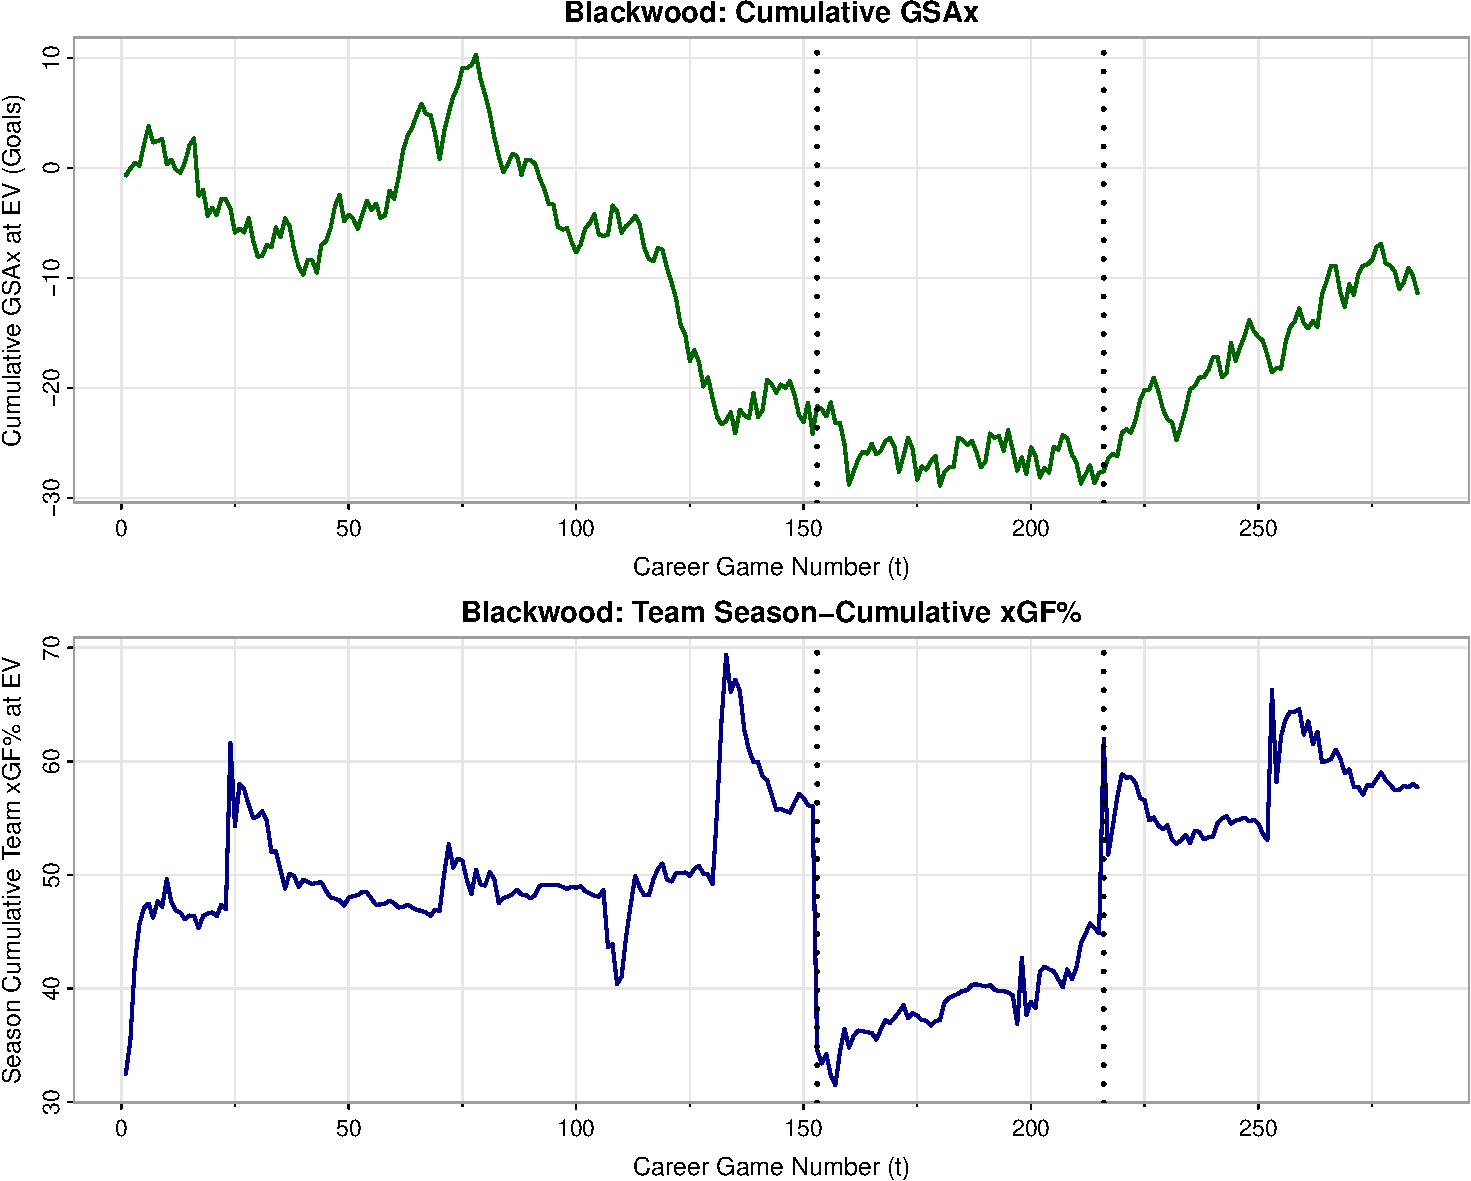
\includegraphics[width=\linewidth]{Presentation1_files/figure-latex/unnamed-chunk-4-1} \end{center}

\begin{Shaded}
\begin{Highlighting}[]
\CommentTok{\# Plot the two Blackwood periodograms used to assess seasonality.}
\NormalTok{op }\OtherTok{\textless{}{-}}\NormalTok{ graphics}\SpecialCharTok{::}\FunctionTok{par}\NormalTok{(}\AttributeTok{no.readonly =} \ConstantTok{TRUE}\NormalTok{)}
\FunctionTok{on.exit}\NormalTok{(graphics}\SpecialCharTok{::}\FunctionTok{par}\NormalTok{(op), }\AttributeTok{add =} \ConstantTok{TRUE}\NormalTok{)}
\NormalTok{graphics}\SpecialCharTok{::}\FunctionTok{par}\NormalTok{(}\AttributeTok{mfrow =} \FunctionTok{c}\NormalTok{(}\DecValTok{1}\NormalTok{, }\DecValTok{2}\NormalTok{), }\AttributeTok{cex.main =} \FloatTok{0.82}\NormalTok{)}
\ControlFlowTok{for}\NormalTok{ (nm }\ControlFlowTok{in} \FunctionTok{c}\NormalTok{(}\StringTok{\textquotesingle{}cumulative\_gsax\_ev\textquotesingle{}}\NormalTok{, }\StringTok{\textquotesingle{}season\_cumulative\_team\_xg\_pct\_ev\textquotesingle{}}\NormalTok{)) \{}
\NormalTok{  info }\OtherTok{\textless{}{-}}\NormalTok{ blackwood\_analysis[[nm]]}\SpecialCharTok{$}\NormalTok{period}
\NormalTok{  title\_text }\OtherTok{\textless{}{-}} \ControlFlowTok{switch}\NormalTok{(}
\NormalTok{    nm,}
    \AttributeTok{cumulative\_gsax\_ev =} \StringTok{\textquotesingle{}Blackwood: Periodogram}\SpecialCharTok{\textbackslash{}n}\StringTok{Cumulative GSAx\textquotesingle{}}\NormalTok{,}
    \AttributeTok{season\_cumulative\_team\_xg\_pct\_ev =} \StringTok{\textquotesingle{}Blackwood: Periodogram}\SpecialCharTok{\textbackslash{}n}\StringTok{Team Season{-}Cumulative xGF\%\textquotesingle{}}
\NormalTok{  )}
\NormalTok{  graphics}\SpecialCharTok{::}\FunctionTok{plot}\NormalTok{(}
\NormalTok{    info}\SpecialCharTok{$}\NormalTok{f,}
\NormalTok{    info}\SpecialCharTok{$}\NormalTok{P,}
    \AttributeTok{type =} \StringTok{\textquotesingle{}l\textquotesingle{}}\NormalTok{,}
    \AttributeTok{main =}\NormalTok{ title\_text,}
    \AttributeTok{xlab =} \StringTok{\textquotesingle{}Frequency\textquotesingle{}}\NormalTok{,}
    \AttributeTok{ylab =} \StringTok{\textquotesingle{}P(frequency)\textquotesingle{}}\NormalTok{,}
    \AttributeTok{col =} \StringTok{\textquotesingle{}navy\textquotesingle{}}\NormalTok{,}
    \AttributeTok{lwd =} \DecValTok{2}
\NormalTok{  )}
\NormalTok{  graphics}\SpecialCharTok{::}\FunctionTok{abline}\NormalTok{(}\AttributeTok{v =}\NormalTok{ info}\SpecialCharTok{$}\NormalTok{freq, }\AttributeTok{col =} \StringTok{\textquotesingle{}red\textquotesingle{}}\NormalTok{, }\AttributeTok{lty =} \DecValTok{2}\NormalTok{, }\AttributeTok{lwd =} \DecValTok{2}\NormalTok{)}
\NormalTok{\}}
\end{Highlighting}
\end{Shaded}

\begin{center}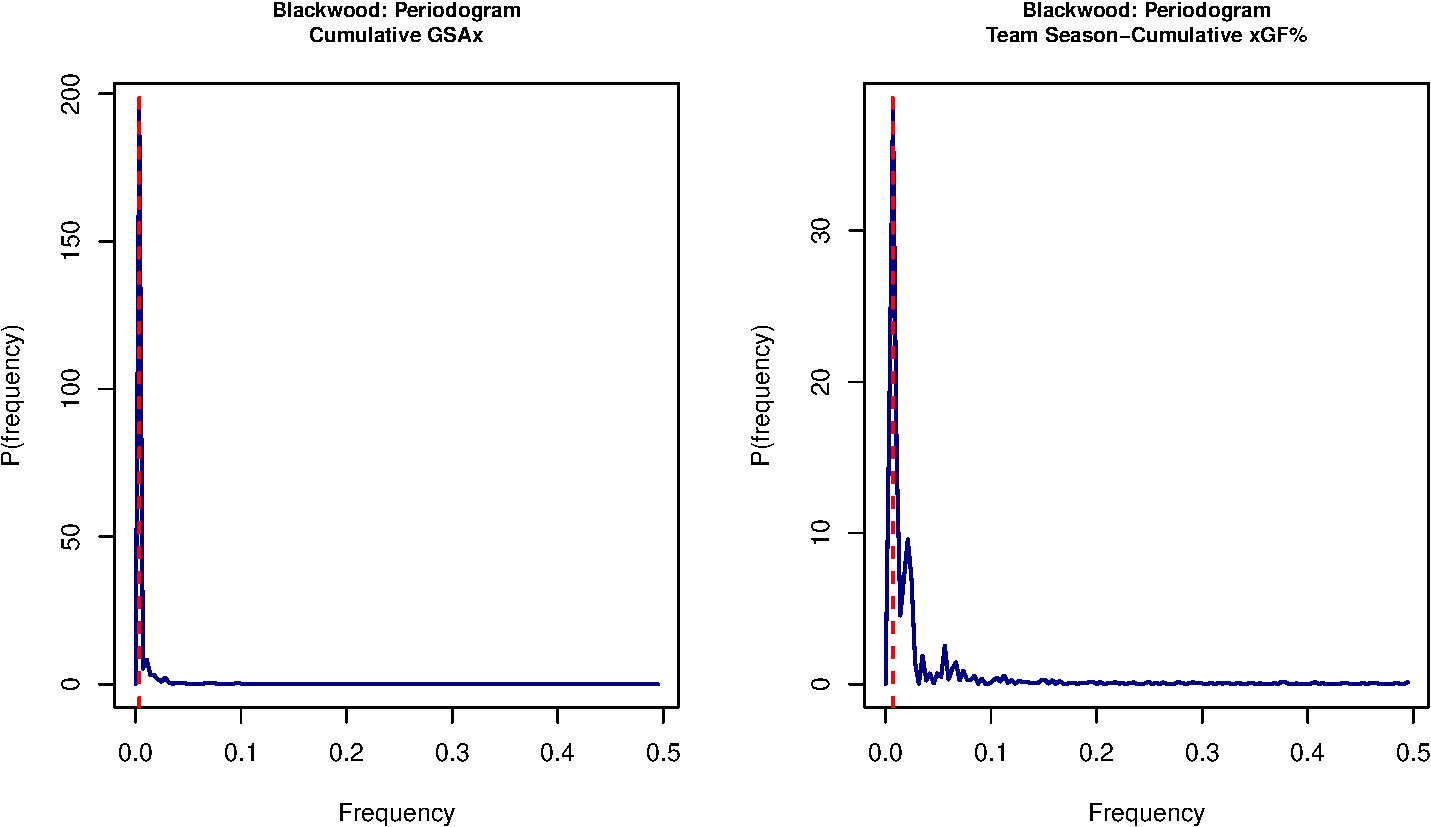
\includegraphics[width=\linewidth]{Presentation1_files/figure-latex/unnamed-chunk-5-1} \end{center}

For Blackwood, neither cumulative series shows convincing seasonality. The \texttt{cumulative\_gsax\_ev} periodogram has a very large spike extremely close to frequency 0, with dominant frequency \(f = 0.003509\) and implied period about 285 games, so it reflects long-run trend rather than a repeating seasonal cycle. The \texttt{season\_cumulative\_team\_xg\_pct\_ev} periodogram peaks at frequency \(f = 0.007018\), which corresponds to about 142.5 games, but that peak is not isolated enough from the rest of the spectrum to support harmonics. Since the team xGF\% series also resets within each season-team segment, its shape is better interpreted as season-to-date team environment rather than a stable repeating cycle. So for Blackwood, I keep only nonseasonal polynomial trend models.

The candidate models for both cumulative Blackwood series are
\[
\begin{aligned}
\text{Model I: } & Y_t = \beta_0 + \beta_1 t + W_t, \\
\text{Model II: } & Y_t = \beta_0 + \beta_1 t + \beta_2 \frac{t^2}{2!} + W_t, \\
\text{Model III: } & Y_t = \beta_0 + \beta_1 t + \beta_2 \frac{t^2}{2!} + \beta_3 \frac{t^3}{3!} + W_t, \\
\text{Model IV: } & Y_t = \beta_0 + \beta_1 t + \beta_2 \frac{t^2}{2!} + \beta_3 \frac{t^3}{3!} + \beta_4 \frac{t^4}{4!} + W_t.
\end{aligned}
\]

\subsection{Blackwood: Cumulative GSAx}\label{blackwood-cumulative-gsax}

\begin{center}
\normalsize

\begin{tabular}{ccccccc}
\toprule
Model & \# Parameters & $R_a^2$ & $p_F$ & AIC & AICc & BIC\\
\midrule
Model I & 2 & 0.4058 & <0.0001 & 7.0666 & 5.2290 & 7.1050\\
Model II & 3 & 0.5716 & <0.0001 & 6.7429 & 4.9055 & 6.7941\\
Model III & 4 & 0.8185 & <0.0001 & 5.8874 & 4.0503 & 5.9515\\
Model IV & 5 & 0.8223 & <0.0001 & 5.8700 & 4.0332 & 5.9469\\
\bottomrule
\end{tabular}
\normalsize
\end{center}\begin{center}
\normalsize

\begin{tabular}{cccccc}
\toprule
Model & ME & MPE & MSE & MAE & MAPE\\
\midrule
Model I & 18.5387 & -152.0291 & 418.3032 & 18.5387 & 152.0291\\
Model II & 30.4078 & -245.2769 & 1084.0513 & 30.4078 & 245.2769\\
Model III & -0.4547 & 11.8134 & 24.6064 & 3.7304 & 29.7550\\
Model IV & -64.6335 & 572.4741 & 6653.5218 & 64.6335 & 572.4741\\
\bottomrule
\end{tabular}
\normalsize
\end{center}

Blackwood's \texttt{cumulative\_gsax\_ev} selects Model III under the Colorado split. Model IV has the best in-sample criteria, but Model III forecasts the Colorado segment much better, with far smaller holdout MSE and MAE. The fitted model is
\[
\widehat{CG}_t = -5.460662 + 0.305395 t - 0.008922 \frac{t^2}{2!} + 0.000072 \frac{t^3}{3!}
\]
where \(CG_t\) is Blackwood's cumulative even-strength GSAx in goals.

\subsection{Blackwood: Season Cumulative Team xGF\%}\label{blackwood-season-cumulative-team-xgf}

\begin{center}
\normalsize

\begin{tabular}{ccccccc}
\toprule
Model & \# Parameters & $R_a^2$ & $p_F$ & AIC & AICc & BIC\\
\midrule
Model I & 2 & 0.0599 & <0.0001 & 6.9011 & 5.0635 & 6.9395\\
Model II & 3 & 0.1921 & <0.0001 & 6.7530 & 4.9156 & 6.8042\\
Model III & 4 & 0.3285 & <0.0001 & 6.5716 & 4.7345 & 6.6357\\
Model IV & 5 & 0.3398 & <0.0001 & 6.5581 & 4.7212 & 6.6350\\
\bottomrule
\end{tabular}
\normalsize
\end{center}\begin{center}
\normalsize

\begin{tabular}{cccccc}
\toprule
Model & ME & MPE & MSE & MAE & MAPE\\
\midrule
Model I & 16.6243 & 28.6982 & 291.5890 & 16.6243 & 28.6982\\
Model II & 28.6238 & 49.5093 & 870.4341 & 28.6238 & 49.5093\\
Model III & 22.9278 & 39.6787 & 547.1849 & 22.9278 & 39.6787\\
Model IV & -7.0585 & -11.8783 & 384.0824 & 14.2241 & 24.6234\\
\bottomrule
\end{tabular}
\normalsize
\end{center}

Blackwood's \texttt{season\_cumulative\_team\_xg\_pct\_ev} selects Model I for forecasting. The higher-order models fit the full sample better, but once the holdout is defined by the Colorado trade, the linear model gives the smallest holdout MSE and MAE by a clear margin. The fitted model is
\[
\widehat{CX}_t = 45.993961 + 0.023823 t
\]
where \(CX_t\) is Blackwood's season-to-date team even-strength xGF\%.

\section{Igor Shesterkin}\label{igor-shesterkin}

\begin{Shaded}
\begin{Highlighting}[]
\CommentTok{\# Plot the two cumulative Shesterkin series.}
\NormalTok{op }\OtherTok{\textless{}{-}}\NormalTok{ graphics}\SpecialCharTok{::}\FunctionTok{par}\NormalTok{(}\AttributeTok{no.readonly =} \ConstantTok{TRUE}\NormalTok{)}
\FunctionTok{on.exit}\NormalTok{(graphics}\SpecialCharTok{::}\FunctionTok{par}\NormalTok{(op), }\AttributeTok{add =} \ConstantTok{TRUE}\NormalTok{)}
\NormalTok{graphics}\SpecialCharTok{::}\FunctionTok{par}\NormalTok{(}\AttributeTok{mfrow =} \FunctionTok{c}\NormalTok{(}\DecValTok{2}\NormalTok{, }\DecValTok{1}\NormalTok{), }\AttributeTok{cex.main =} \FloatTok{0.95}\NormalTok{)}
\NormalTok{astsa}\SpecialCharTok{::}\FunctionTok{tsplot}\NormalTok{(}
\NormalTok{  stats}\SpecialCharTok{::}\FunctionTok{ts}\NormalTok{(shesterkin\_gbgs}\SpecialCharTok{$}\NormalTok{cumulative\_gsax\_ev, }\AttributeTok{start =} \DecValTok{1}\NormalTok{, }\AttributeTok{frequency =} \DecValTok{1}\NormalTok{),}
  \AttributeTok{main =} \StringTok{\textquotesingle{}Shesterkin: Cumulative GSAx\textquotesingle{}}\NormalTok{,}
  \AttributeTok{xlab =} \StringTok{\textquotesingle{}Career Game Number (t)\textquotesingle{}}\NormalTok{,}
  \AttributeTok{ylab =} \StringTok{\textquotesingle{}Cumulative GSAx at EV (Goals)\textquotesingle{}}\NormalTok{,}
  \AttributeTok{col =} \StringTok{\textquotesingle{}darkgreen\textquotesingle{}}\NormalTok{,}
  \AttributeTok{lwd =} \DecValTok{2}
\NormalTok{)}

\NormalTok{astsa}\SpecialCharTok{::}\FunctionTok{tsplot}\NormalTok{(}
\NormalTok{  stats}\SpecialCharTok{::}\FunctionTok{ts}\NormalTok{(shesterkin\_gbgs}\SpecialCharTok{$}\NormalTok{season\_cumulative\_team\_xg\_pct\_ev, }\AttributeTok{start =} \DecValTok{1}\NormalTok{, }\AttributeTok{frequency =} \DecValTok{1}\NormalTok{),}
  \AttributeTok{main =} \StringTok{\textquotesingle{}Shesterkin: Team Season{-}Cumulative xGF\%\textquotesingle{}}\NormalTok{,}
  \AttributeTok{xlab =} \StringTok{\textquotesingle{}Career Game Number (t)\textquotesingle{}}\NormalTok{,}
  \AttributeTok{ylab =} \StringTok{\textquotesingle{}Season Cumulative Team xGF\% at EV\textquotesingle{}}\NormalTok{,}
  \AttributeTok{col =} \StringTok{\textquotesingle{}navy\textquotesingle{}}\NormalTok{,}
  \AttributeTok{lwd =} \DecValTok{2}
\NormalTok{)}
\end{Highlighting}
\end{Shaded}

\begin{center}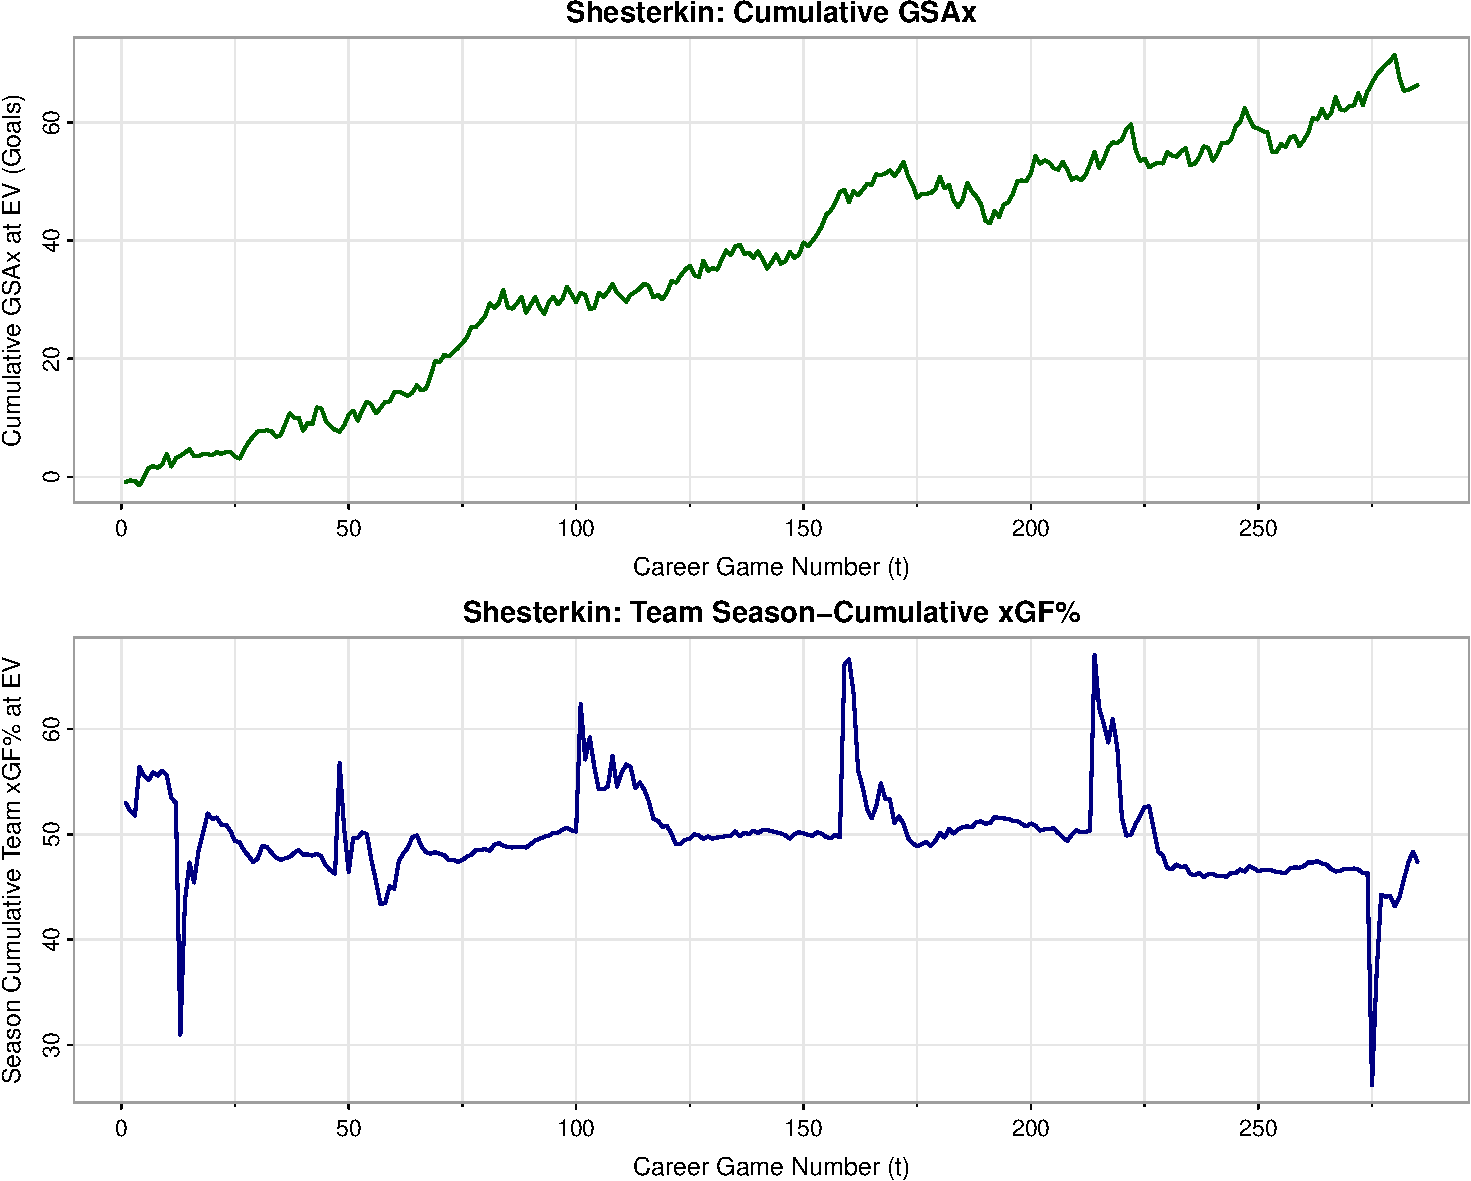
\includegraphics[width=\linewidth]{Presentation1_files/figure-latex/unnamed-chunk-8-1} \end{center}

\begin{Shaded}
\begin{Highlighting}[]
\CommentTok{\# Plot the two Shesterkin periodograms.}
\NormalTok{op }\OtherTok{\textless{}{-}}\NormalTok{ graphics}\SpecialCharTok{::}\FunctionTok{par}\NormalTok{(}\AttributeTok{no.readonly =} \ConstantTok{TRUE}\NormalTok{)}
\FunctionTok{on.exit}\NormalTok{(graphics}\SpecialCharTok{::}\FunctionTok{par}\NormalTok{(op), }\AttributeTok{add =} \ConstantTok{TRUE}\NormalTok{)}
\NormalTok{graphics}\SpecialCharTok{::}\FunctionTok{par}\NormalTok{(}\AttributeTok{mfrow =} \FunctionTok{c}\NormalTok{(}\DecValTok{1}\NormalTok{, }\DecValTok{2}\NormalTok{), }\AttributeTok{cex.main =} \FloatTok{0.82}\NormalTok{)}
\ControlFlowTok{for}\NormalTok{ (nm }\ControlFlowTok{in} \FunctionTok{c}\NormalTok{(}\StringTok{\textquotesingle{}cumulative\_gsax\_ev\textquotesingle{}}\NormalTok{, }\StringTok{\textquotesingle{}season\_cumulative\_team\_xg\_pct\_ev\textquotesingle{}}\NormalTok{)) \{}
\NormalTok{  info }\OtherTok{\textless{}{-}}\NormalTok{ shesterkin\_analysis[[nm]]}\SpecialCharTok{$}\NormalTok{period}
\NormalTok{  title\_text }\OtherTok{\textless{}{-}} \ControlFlowTok{switch}\NormalTok{(}
\NormalTok{    nm,}
    \AttributeTok{cumulative\_gsax\_ev =} \StringTok{\textquotesingle{}Shesterkin: Periodogram}\SpecialCharTok{\textbackslash{}n}\StringTok{Cumulative GSAx\textquotesingle{}}\NormalTok{,}
    \AttributeTok{season\_cumulative\_team\_xg\_pct\_ev =} \StringTok{\textquotesingle{}Shesterkin: Periodogram}\SpecialCharTok{\textbackslash{}n}\StringTok{Team Season{-}Cumulative xGF\%\textquotesingle{}}
\NormalTok{  )}
\NormalTok{  graphics}\SpecialCharTok{::}\FunctionTok{plot}\NormalTok{(}
\NormalTok{    info}\SpecialCharTok{$}\NormalTok{f,}
\NormalTok{    info}\SpecialCharTok{$}\NormalTok{P,}
    \AttributeTok{type =} \StringTok{\textquotesingle{}l\textquotesingle{}}\NormalTok{,}
    \AttributeTok{main =}\NormalTok{ title\_text,}
    \AttributeTok{xlab =} \StringTok{\textquotesingle{}Frequency\textquotesingle{}}\NormalTok{,}
    \AttributeTok{ylab =} \StringTok{\textquotesingle{}P(frequency)\textquotesingle{}}\NormalTok{,}
    \AttributeTok{col =} \StringTok{\textquotesingle{}navy\textquotesingle{}}\NormalTok{,}
    \AttributeTok{lwd =} \DecValTok{2}
\NormalTok{  )}
\NormalTok{  graphics}\SpecialCharTok{::}\FunctionTok{abline}\NormalTok{(}\AttributeTok{v =}\NormalTok{ info}\SpecialCharTok{$}\NormalTok{freq, }\AttributeTok{col =} \StringTok{\textquotesingle{}red\textquotesingle{}}\NormalTok{, }\AttributeTok{lty =} \DecValTok{2}\NormalTok{, }\AttributeTok{lwd =} \DecValTok{2}\NormalTok{)}
\NormalTok{\}}
\end{Highlighting}
\end{Shaded}

\begin{center}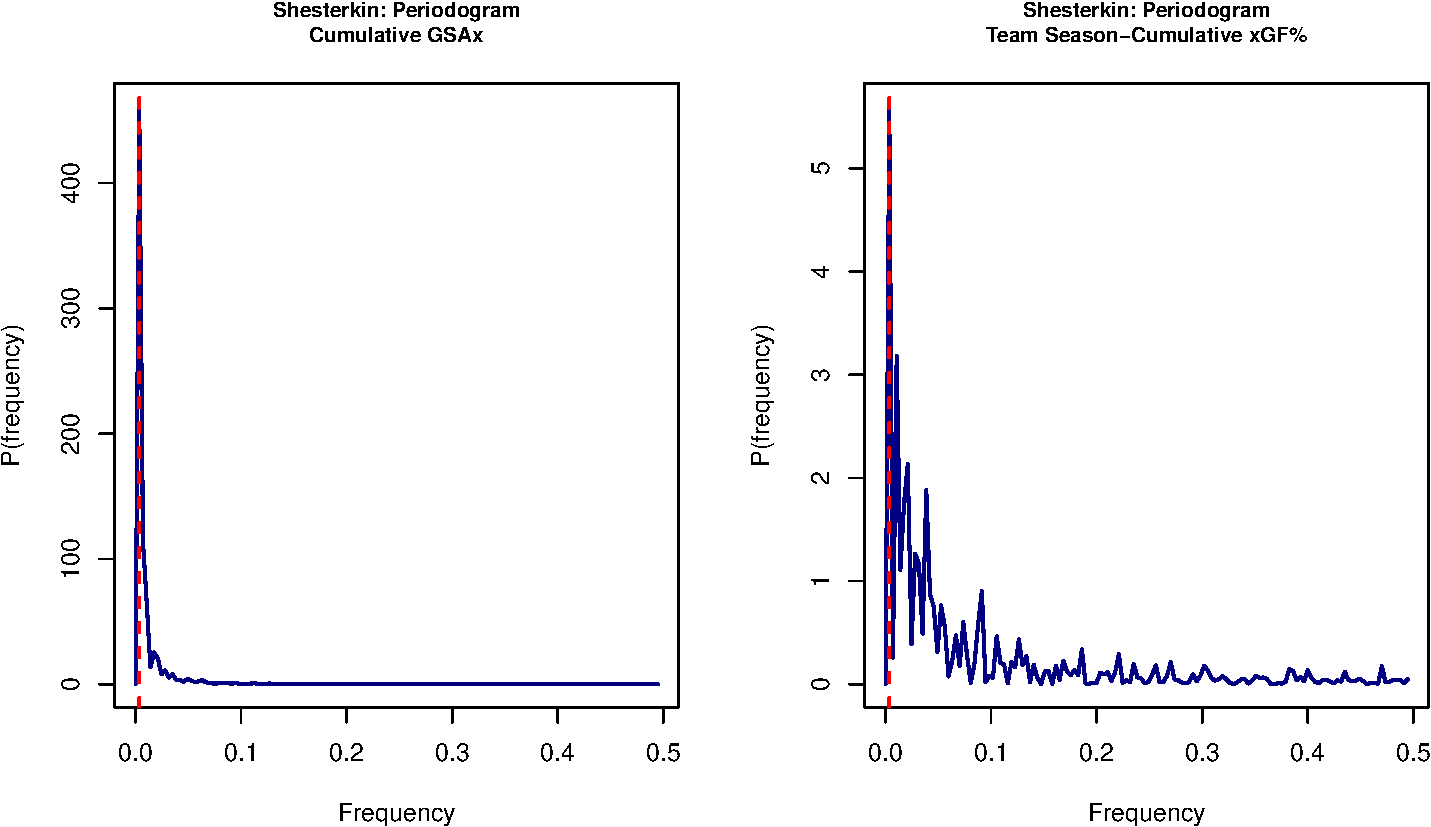
\includegraphics[width=\linewidth]{Presentation1_files/figure-latex/unnamed-chunk-9-1} \end{center}

For Shesterkin, the same conclusion holds: there is no convincing seasonality in either cumulative series. The \texttt{cumulative\_gsax\_ev} periodogram again has its strongest spike extremely close to frequency 0, while the \texttt{season\_cumulative\_team\_xg\_pct\_ev} periodogram has its strongest peak at frequency \(f = 0.003509\), corresponding to about 285 games. That peak is not cleanly separated enough from the surrounding spectrum to justify harmonics, and the season-to-date construction itself creates broad low-frequency structure rather than a clean repeating cycle. So I again keep only nonseasonal polynomial trend models.

\subsection{Shesterkin: Cumulative GSAx}\label{shesterkin-cumulative-gsax}

\begin{center}
\normalsize

\begin{tabular}{ccccccc}
\toprule
Model & \# Parameters & $R_a^2$ & $p_F$ & AIC & AICc & BIC\\
\midrule
Model I & 2 & 0.9593 & <0.0001 & 5.6224 & 3.7848 & 5.6608\\
Model II & 3 & 0.9771 & <0.0001 & 5.0492 & 3.2118 & 5.1004\\
Model III & 4 & 0.9773 & <0.0001 & 5.0458 & 3.2086 & 5.1098\\
Model IV & 5 & 0.9812 & <0.0001 & 4.8584 & 3.0215 & 4.9353\\
\bottomrule
\end{tabular}
\normalsize
\end{center}\begin{center}
\normalsize

\begin{tabular}{cccccc}
\toprule
Model & ME & MPE & MSE & MAE & MAPE\\
\midrule
Model I & -8.0143 & -13.6854 & 73.3677 & 8.0180 & 13.6916\\
Model II & 0.5612 & 0.5564 & 11.2062 & 2.7151 & 4.4855\\
Model III & 9.8773 & 15.8069 & 152.3764 & 9.8773 & 15.8069\\
Model IV & 0.2655 & 0.2747 & 6.0653 & 1.8962 & 3.1813\\
\bottomrule
\end{tabular}
\normalsize
\end{center}

Shesterkin's \texttt{cumulative\_gsax\_ev} selects Model IV. Here the quartic model is favored by the in-sample criteria and also by the aligned holdout MSE and MAE, so the model choice is cleaner than it is for Blackwood. The fitted model is
\[
\widehat{CG}_t = -0.069001 + 0.127717 t + 0.006883 \frac{t^2}{2!} - 0.000132 \frac{t^3}{3!} + 0.000001 \frac{t^4}{4!}
\]
where \(CG_t\) is Shesterkin's cumulative even-strength GSAx in goals.

\subsection{Shesterkin: Season Cumulative Team xGF\%}\label{shesterkin-season-cumulative-team-xgf}

\begin{center}
\normalsize

\begin{tabular}{ccccccc}
\toprule
Model & \# Parameters & $R_a^2$ & $p_F$ & AIC & AICc & BIC\\
\midrule
Model I & 2 & 0.0242 & 0.0049 & 5.6900 & 3.8524 & 5.7284\\
Model II & 3 & 0.1563 & <0.0001 & 5.5481 & 3.7107 & 5.5994\\
Model III & 4 & 0.2490 & <0.0001 & 5.4351 & 3.5980 & 5.4992\\
Model IV & 5 & 0.2773 & <0.0001 & 5.4002 & 3.5634 & 5.4771\\
\bottomrule
\end{tabular}
\normalsize
\end{center}\begin{center}
\normalsize

\begin{tabular}{cccccc}
\toprule
Model & ME & MPE & MSE & MAE & MAPE\\
\midrule
Model I & -5.3379 & -12.4855 & 50.0461 & 6.2031 & 13.9370\\
Model II & -6.3993 & -14.7947 & 64.7149 & 7.1874 & 16.1127\\
Model III & 2.8610 & 5.5471 & 25.8931 & 3.8753 & 8.3711\\
Model IV & -27.5100 & -61.6650 & 1149.1469 & 28.1081 & 62.6637\\
\bottomrule
\end{tabular}
\normalsize
\end{center}

Shesterkin's \texttt{season\_cumulative\_team\_xg\_pct\_ev} selects Model III. Model IV has the best in-sample criteria, but Model III gives the smallest holdout MSE and MAE, so it is the better practical forecasting choice under the aligned split. The fitted model is
\[
\widehat{CX}_t = 51.028875 - 0.080546 t + 0.002015 \frac{t^2}{2!} - 0.000018 \frac{t^3}{3!}
\]
where \(CX_t\) is Shesterkin's season-to-date team even-strength xGF\%.

\section{Preliminary Conclusion}\label{preliminary-conclusion}

These results are only preliminary, but they already suggest a useful contrast. For both goalies, cumulative GSAx requires a curved trend, while the season-to-date team xGF\% series is more tied to within-season team environment and resets when a new season or team segment begins. Relative to Shesterkin's steadier one-team path, Blackwood's cumulative GSAx is more visibly shaped by franchise changes, and the Colorado split materially affects which cumulative GSAx model forecasts best. So at this stage, the presentation evidence does not prove that GSAx is fully team-independent; instead, it suggests that long-run goalie results and season-level team environment can evolve differently across the two goalies, especially when one goalie experiences major franchise changes and the other does not.

\end{document}
